\chapter{Chronos hardware}

This chapter describes the hardware constituting a Chronos watch kit,
as offered by Texas Instruments. The applications that can be deployed
on the watch are limited by the capabilities of the hardware.
Therefore, understanding what the hardware can do is essential to
understand what applications are possible.

\section{The eZ430-Chronos package}

eZ430 Chronos was meant as a reference platform for wireless mobile
systems.  It is a versatile, highly integrated smart watch.  According
to the manufacturer, Texas Instruments, it was designed  as an
evaluation platform for developers.  Although it is not intended for
the consumer market, it is widely available and popular among
technology hobbyists.

eZ430 is sold in a box that contains the actual watch, a USB programing dongle
and a USB radio dongle, along with a software CD and a screw driver.
These are shown in Figures \ref{fig:chronos_kit} and
\ref{fig:chronos_watch}.

\begin{figure}[h]
  \centering
  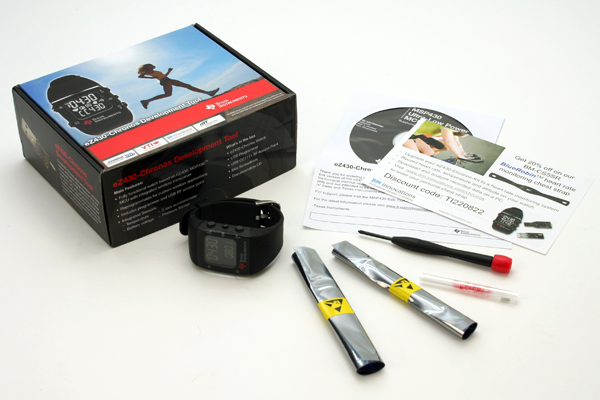
\includegraphics[width=0.7\textwidth]{img/chronos_kit.jpg}
  \caption{Chronos kit. (Courtesy Marc de
  Vinck)}
  \label{fig:chronos_kit}
\end{figure}

\begin{figure}[h]
  \centering
  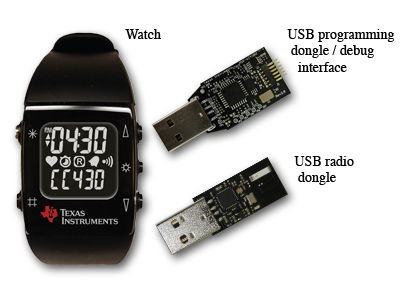
\includegraphics[width=0.6\textwidth]{img/chronos_watch.png}
  \caption{Main elements of the Chronos kit. (Courtesy of Texas
  Instruments)}
  \label{fig:chronos_watch}
\end{figure}

\section{Elements of the watch}
A Chronos watch is battery powered and has a typical wrist strap that
allows for wearing it like any other watch. Its uniqueness, however,
comes from what lies within the housing. Of the more common elements
it has a {\bf 96 segment LCD display}, which includes two rows of
digits, respectively 4 and 5 digits long, and many other symbols. All
segments can be lit (and even blinked) independently.  This allows the
watch to display crude letters along with numbers. The available LCD
segments are shown in Figure \ref{fig:chronos_segs}.  The watch also
has 5 programmable buttons, one of which controls the screen
back-light.

\begin{figure}[h]
  \centering
  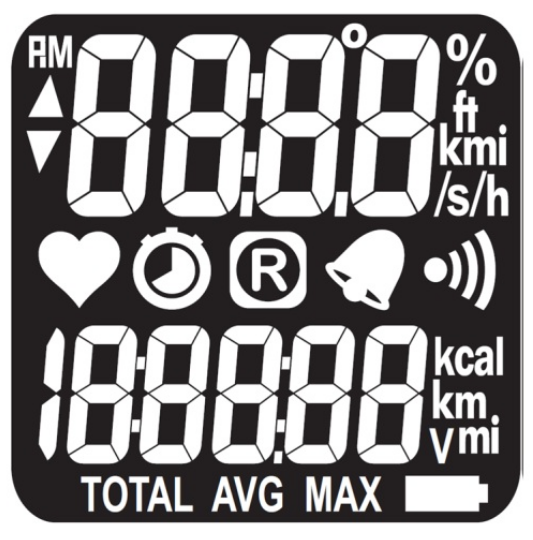
\includegraphics[width=0.4\textwidth]{img/chronos_segs.png}
  \caption{All segments of the watch. (Courtesy Texas
  Instruments)}
  \label{fig:chronos_segs}
\end{figure}

A less common element is a fully programmable MCU ({\bf Mobile Compute
Unit}), labeled CC430F6137. It is a so called system-on-chip (or
SoC), because it contains a built-in {\bf radio transceiver}.
Conveniently, it uses the 868 MHz radio band for which no license is
required. The MCU is discussed in more detail in the next section.

Moreover, the watch has some on-board sensors: an {\bf accelerometer}
and a {\bf temperature and pressure sensor}. The accelerometer can
detect the watch's position relative to the Earth's gravity, can notice a
sudden motion, and can detect if the watch is falling. The thermometer
simply measures the current air temperature, with a $1^{\circ}$C
accuracy. The pressure, in turn, is precise enough to measure even a
0.3 meter change in altitude, which is sufficient to detect on which
floor of a building the watch is. For this reason, the pressure sensor
is often called an {\bf altimeter}.

Finally, the watch casing is water resistant up to 30 meters and hosts
typical CR2032 coin-cell batteries, which have a maximal capacity of
225 mAh and provide a nominal voltage of 3.0 V.

\section{Mobile Compute Unit}

MCU is a Compute Programmable Unit (CPU) designed for extremely
low power usage. The one used in Chronos has the MSP430 (Mixed Signal
microProcessor) architecture, which is particularly suited for
low-power applications. It belongs to the TI family of products
codenamed CC430, which features 16-bit, RISC-based (Reduced Instruction
Set Computing) CPUs \cite{CC430ds}. The exact chip soldered in the
watch is CC430F6137 \cite{CC430F6137ds}.

Applications that may be run on the watch are limited by the MCU's
resources. One of the most constrained resources is memory. There are two types
of memory available:
\begin{itemize}
  \item {\bf 32KB of flash memory}. This is non-volatile fast-read
    slow-write on-chip memory. It stores code and data. After a reset,
    the MCU jumps to a predefined location (address 0x8000) in this
    memory and starts executing instructions recorded there. Although
    the 32KB of flash may seem little, with modern code-size
    optimizing compilers, quite complex applications are possible. For
    example, 32KB is just enough to fit a temperature monitoring
    application in which each node sends out its readings and forwards
    readings of other nodes to a single sink node.
  \item {\bf 4KB of RAM}. It is similar to PC RAM and its
    operation consumes a lot of energy. That's why its amount is so
    small. 4KB is, however, just enough to fit the temperature monitoring
    application mentioned above.
\end{itemize}

The MCU clock is scalable and can run at the {\bf maximum frequency of
20 MHz}.  MSP430 RISC instructions are, however, much simpler than, for
example, x86 ones. To illustrate this difference, a 16 MHz CC430 (default
in Chronos) was compared to an Intel Core 2 x86 processor clocked at
2.53 GHz, with an implementation of the Floyd-Warshal
algorithm\footnote{Actually a smaller array was used, because $300^2$
exceeds memory available on the watch.} as the benchmark.

\begin{lstlisting}[numbers=none, keywordstyle=\bfseries, language=C]
    enum { N = 300 };
    uint16_t M[N*2];

    void floydWarshal() {
        uint16_t k, i, j;
        for (k = 0; k < N; k++)
          for (i = 0; i < N; i++)
            for (j = 0; j < N; j++) {
                if (M[i+j] > M[i+k] + M[k+j])
                  M[i+j] = M[i+k] + M[k+j];
            }
    }
\end{lstlisting}

Execution of the algorithm took 27s on the watch while on the PC the
time was only 40ms.  To make a fair comparison, we must scale down the
PC clock to 16MHz. If it were so, the execution would take 6.3
seconds. Overall, the watch MCU is approximately 4 times less
efficient due to sole architectural differences from an ordinary x86.
If we also count in the clock speed difference, the watch is over 670
times slower than a PC. While the comparison is crude, it gives an
intuition on the processing performance of the watch.

In the same way we can compare power consumption.  The Intel CPU uses
approximately 15W of power, while the watch MCU only 11mW. If we
scaled the MCU up to the PC clock speed it would only use 1.7W. In
other words, the MCU is much more power efficient, which is in line
with its main function: a low power watch.

\section{Additional hardware functions}
\label{ch:hardware_functions}

There are certain functions that, though possible to be implemented in
software, are also easily implementable in hardware. Choosing the
hardware approach saves both execution time and energy. Moreover, some
features can be implemented only with hardware support. Let us discuss
the most important hardware features available in the CC430f6137 MCU
(and many other members of the CC430 family for that matter).

{\bf LPM (Low Power Mode) support} allows an MCU to dynamically switch to
one of a few power states.  They are called Active, LPM0, LPM1, etc.
Each successive one consumes less energy by disabling more hardware
functions and peripherals. This mechanism is crucial for lengthening
the battery life. To illustrate how important this is, let us present
some crude battery life estimates:

\begin{itemize}
    \item In Active mode (executing instructions), the watch's battery
      would last for a week (6.8 days).
    \item In LPM0 or LPM1 the battery life would grow to roughly 280 days.
    \item In LPM2 the battery would last around 9 years.
    \item And finally in LPM3 or LPM4 it would last half a decade (52
    years), which is more than the battery's shelf-life.
\end{itemize}
If a battery is to last years, an MCU must spend most of its time in
the lowest power modes.

For this reason, another vital subsystem is {\bf Timer\_A}, which
allows for setting an alarm that will fire (interrupt) after a specific
period of time (on the order of milliseconds) and execute a certain
piece of code (an interrupt handler). It would be impossible to use low
power modes without such functionality.

Since Chronos is primarily a watch, {\bf RTC\_A (Real Time Clock)} is
an another vital component. This module provides wall clock and
calendar functions. It is the means for accessing seconds, minutes,
hours, days of week, days of month, months, and years.  Moreover it
can also be configured as a general-purpose counter --- something
similar to Timer\_A.

The MCU has 64 pins. Most of them are {\bf IO pins}. They can be
configured to act as an input, output or special function.  In input
mode, they inform of the signal that's connected to them (high or
low). Similarly, in output mode, they can generate a high or low
signal \footnote{If one were tempted to connect input and output pins
to experiment with signal passing, if careless, he could destroy the
MCU.  An output pin produces a maximum of several mA of current. An
input pin would then accept all this current. In effect, such a
connection without a resistor would result in a short circuit {\bf
through the chip}. Using a 2k $\Omega$ resistor can alleviate the
problem.}. Special function mode connects the pin to an internal
hardware component, for example, the LCD driver.  Also it is possible
to be notified (via interrupt) if the state of an input pin changes.
This enables, for instance, implementing button drivers.

There are more LCD segments on the display than there are pins on the
chip. Even if there were enough, using so many pins for the LCD would
be wasteful. It's better to spread data over time. In a technique
called multiplexing, the chip selects a group of segments by powering
a control pin and lits the ones within the selected group. Eight group
pins and eight element pins are enough to drive 64 LCD segments in
this fashion. Groups are changed quickly enough that a human doesn't
notice any blinking, which makes it a practical solution.  However,
implementing this in software would be wasteful, therefore {\bf
LCD\_B} driver does all this in hardware.

Another vital hardware driver is {\bf USCI (Universal Serial
Communication Interface)}. It can be configured to pose as one of
standardized communication interfaces. Most notably these are SPI
(Serial Peripheral Interface), I$^2$C (Inter-Integrated Circuit) and
UART (Universal Asynchronous Receiver/Transmitter). Though cumbersome,
each one can be implemented in software. However, hardware support
increases performance by an order of magnitude. UART, for example, is
particularly important during development, because it allows for sending
text from the watch's MCU to a PC.

An interesting and practical feature of the CC430 family is the
ability to do {\bf port remapping} at runtime. Typically, special
functions are hard-connected to certain chip pins. For example UART's
Tx and Rx may be mapped to pins P1.0 and P1.1. If we had two
components that wanted to communicate with the MCU chip via UART, some
external circuitry would be needed to reconnect the pins on demand.
This isn't, however, necessary in the CC430 family, because such
functionality is built-in. Hardware drivers can be reconnected to
arbitrary IO pins without powering down the MCU.

The following two hardware features are related to data integrity and
security. The first one is a {\bf CRC module} that speeds up
calculation of check sums.  MSP430 MCUs are poor in doing certain
types of operations like shifts and using this hardware leads to
considerable speed improvements, especially on large data blocks.

The second one is the {\bf AES128 Accelerator}. Advanced Encryption
Standard 128 is a secure symmetric cipher. Its complicated
encryption and decryption algorithms were implemented in hardware.

Finally, the following three hardware functions ease the interaction
of the MCU with analog circuits.  {\bf REF} is a reference voltage
generator. Some components, like the LCD, require a certain electric
voltage for their operation.  Others perform comparisons of external
voltages to a reference voltage. It is convenient to generate such
reference voltages without the help from any external circuitry.

{\bf Comp\_B} is a voltage comparator. It is a circuit that can
compare two voltages and tell which one is higher. Moreover one of
them can be a reference voltage of a known value. Comparators are used
to interface analog signals to digital circuitry.

And finally {\bf ADC12\_A} is an analog to digital converter
module. Conceptually it's a generalized comparator \footnote{In
fact ADC is implemented using several comparators, with varying
reference voltages.}, because it returns multiple bits of information
instead of one.  An ADC circuit can very quickly measure the value of
some external voltage. Therefore, if you wanted to construct a thermometer
you would connect a thermistor (resistance of which reflects its
temperature) to a reference voltage and measure the resulting
voltage with ADC. From that, temperature would be derived.

There are also some subsystems that support development and in field
operation. The {\bf Watchdog Timer} is a circuit that breaks infinite
loops and other MCU hangs. It needs to be refreshed periodically,
otherwise it will reset the device.

The {\bf bootstrap loader}, in turn, holds an additional operating
system on the device.  Most notably, it can be designed to allow for
software updates through the radio or UART.

\section{Radio transceiver}

In the past, radio transceivers typically comprised separate chips. In
our case, however, such a chip, called CC1101, has been integrated into
the CC430F6137 MCU.  It operates on the unlicensed 868 MHz band
\footnote{However, the European Telecommunications Standards Institute
limits the duty cycle and maximal power output on the 868 MHz band.}.
The module is capable of sending and receiving short packets of
data\footnote{Typically up to 63 bytes long, but through software, it
is possible to support longer packets. Theoretically even $2^{16}$
bytes long.}.  The radio module is usually the most power consuming
component and CC1101 is not an exception. Therefore, it is important
to keep it off as much as possible.

\section{Other devices included in the kit}

For the developer, an important component is the {\bf USB debug
interface}. It allows for:
\begin{itemize}
  \item Programing the watch with a binary image (a .hex or .exe file).
  \item Receiving text (printf messages) through UART \footnote{A small
    hardware modification is necessary for that. It's described in
    Appendix \ref{appendix:uart_pins}.}.
  \item Connecting to the watch with a debugger. In particular, the
    developer can view the program execution, memory and registers in
    the Eclipse IDE.
\end{itemize}
A connection of the debug interface with the watch is shown in Figure
\ref{fig:chronos_dongle}.

\begin{figure}[h]
  \centering
  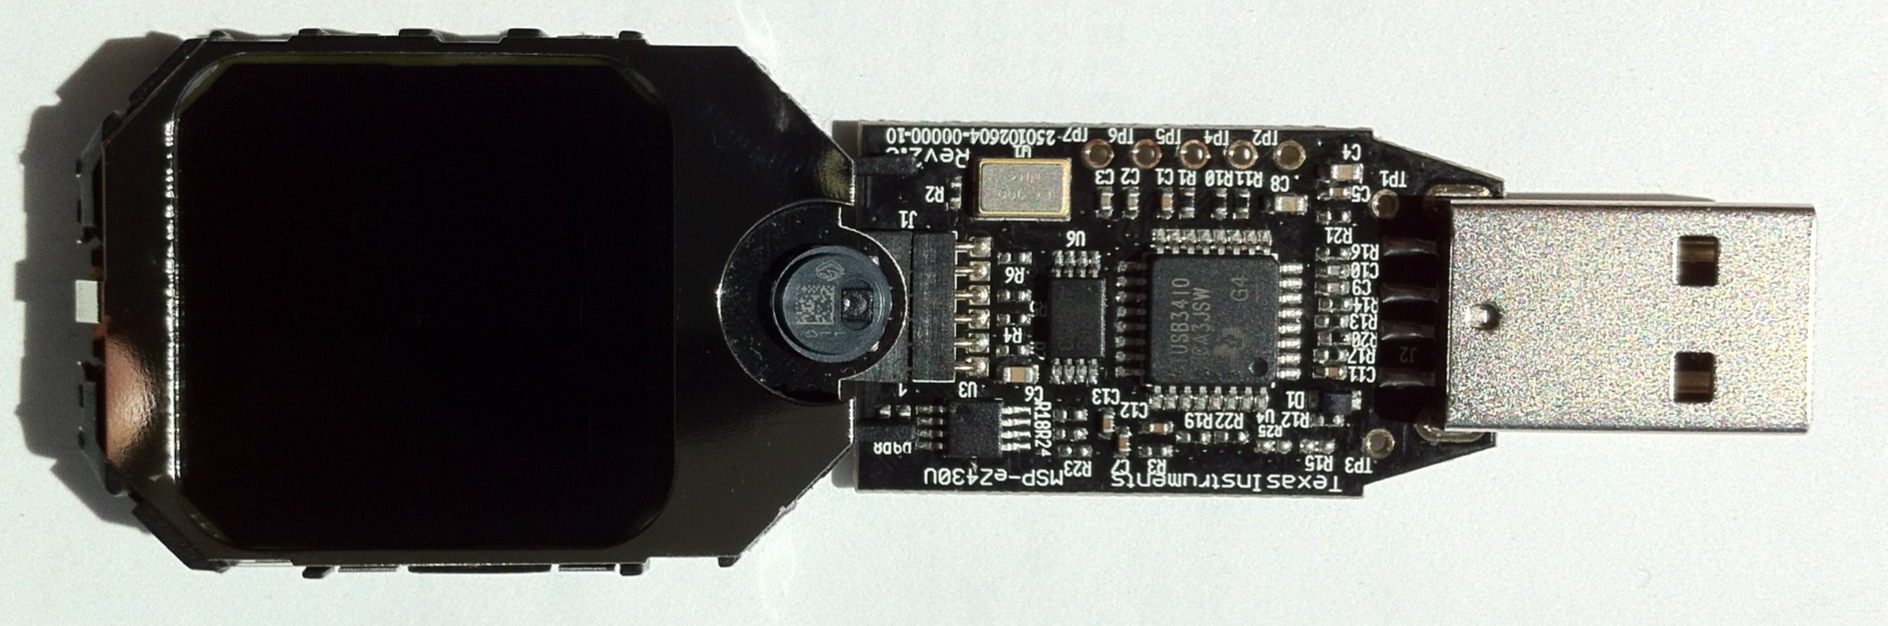
\includegraphics[width=0.8\textwidth]{img/chronos_dongle.jpg}
  \caption{Watch connected to the debug interface.}
  \label{fig:chronos_dongle}
\end{figure}

Another supporting device is the {\bf USB RF access point dongle},
which can communicate with the watch over the radio and also forward
its commands to the PC. One example use is driving a PC mouse by
moving the watch or controlling a presentation with the watch's
buttons. In fact, the dongle also uses a system-on-chip MCU, which
additionally has USB support. However, its architecture is different
from MSP430 and currently unsupported by TinyOS. Programming it is an
interesting future work.

The dongle is shown in Figure \ref{fig:chronos_rfdongle}.

\begin{figure}[h]
  \centering
  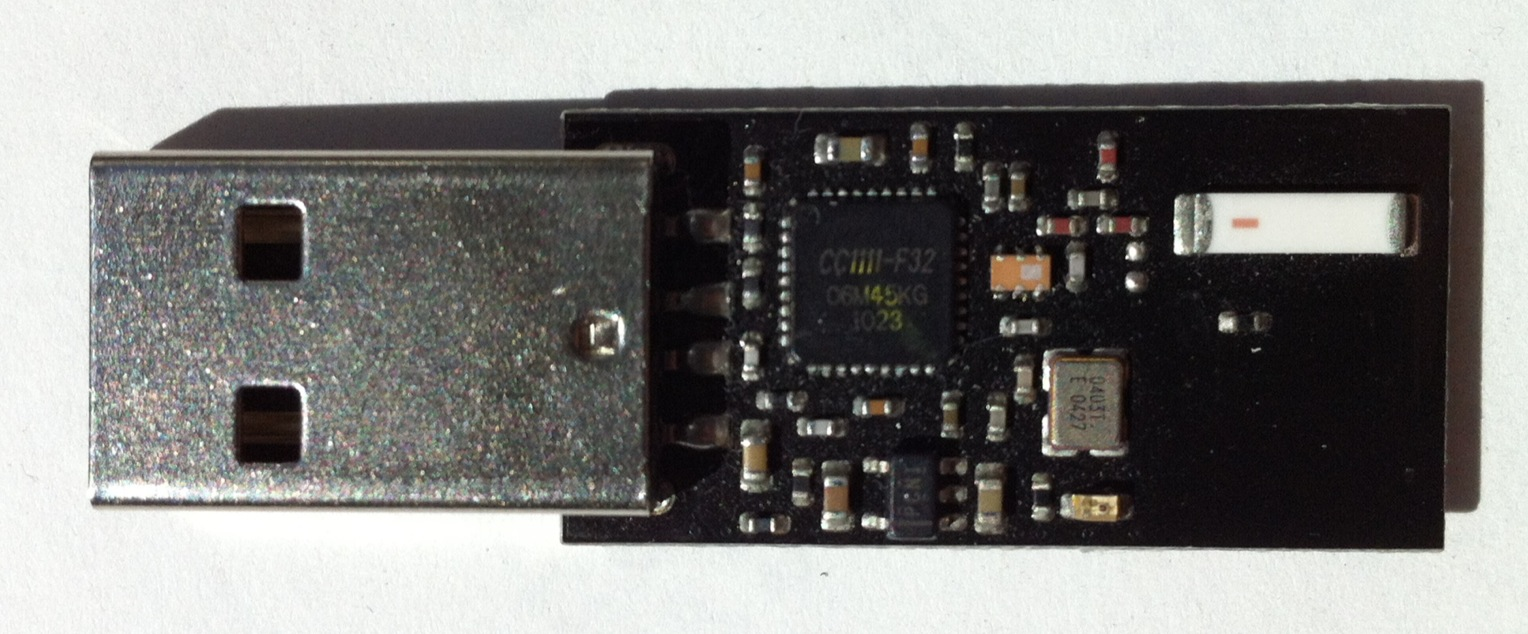
\includegraphics[width=0.6\textwidth]{img/chronos_rfdongle.jpg}
  \caption{USB RF access point dongle.}
  \label{fig:chronos_rfdongle}
\end{figure}

\section{Intended use of the watch}

\subsection{Factory firmware}

Texas Instruments provides a software example that is preloaded on every
watch. It provides standard watch functions like time, date, alarm and
stopwatch. Also it shows averaged sensor measurements: altitude,
acceleration, battery voltage and temperature. If an external  heart
rate monitor is present the watch will also display its readings. For
the radio communication, there are three wireless modes:

\begin{itemize}
  \item ACC --- transmit accelerometer motion data.
  \item PPT --- wireless presentation control or bind Chronos
    keys to PC keyboard shortcuts.
  \item Sync --- syncs time and date with PC and calibrates
    temperature and altitude.
\end{itemize}

\subsection{Community use cases}
There are many programs written by technology enthusiasts. Some of the
examples include:

\begin{itemize}
  \item wireless door lock --- a system, of two devices, with which it
    is possible to define a password as a gesture recognized by the
    accelerometer.
  \item flying mouse --- move watch and use it as a PC mouse.
  \item automatic lighting system --- control light bulbs from your
    watch.
  \item Time-based One Time Password (TOTP) Authenticator --- provides
    token based authentication system.
\end{itemize}

\subsection{Shortcomings of existing software}

Applications written for Chronos tend to be simple: examples above
confirm that. Typically, they are written by one person to perform a
particular task and share little or no code at all.  While it would be
beneficial if a common software platform emerged from these efforts,
nothing like this has happened. Moreover, the applications listed
above leverage none of the advanced algorithms published in
scientific papers. A Chronos watch is, in essence, a mobile wireless
sensor node and not utilizing research that has been done in
that field is wasteful. One may expect much more from this platform.

In our view, there are three main difficulties that contribute to this
situation.  Firstly, watch software development is very different from
what developers are used to on PCs. There is no operating system
that would create abstractions of the underlying hardware, like
multitasking, data persistence, memory protection and process resource
management.  Likewise, the inability to run the developed application side by
side with debugging tools makes it more cumbersome to trace problems.
Furthermore, the limited resources on the MCU, most notably power, require writing more
complicated code, of which managing the MCU power states is a good example.
Libraries could alleviate this problem, but without a solid software
platform, it's difficult to create them. In effect, the developer is forced
to write both an application and operating system.

Secondly, the C language, which apart from the assembly is the only
language supported by MSP430 compilers,  itself makes it difficult to
manage larger projects. Basically all names are in a global name
space, there are no boundaries between components and it encourages
poor programing practises, like register bit manipulation without any
comments.

Thirdly, working directly with the hardware, creates many new
opportunities for errors. Most common ones include race conditions during
interrupt handling, memory access violations and leaks, omitted or
doubled initialization and improper use of hardware.  Moreover, in any
reasonably complex application, there is a need for some form of
concurrency.  Implementing it from scratch is difficult and often
causes many additional programming errors.

Our thesis aims to alleviate the above shortcomings. To this end we
employ the NesC programming language and the TinyOS operating system.


% Vim settings:
% vim: set textwidth=70:
% vim: set fo+=t:
